\documentclass[11pt,]{article}
\usepackage{lmodern}
\usepackage{amssymb,amsmath}
\usepackage{ifxetex,ifluatex}
\usepackage{fixltx2e} % provides \textsubscript
\ifnum 0\ifxetex 1\fi\ifluatex 1\fi=0 % if pdftex
  \usepackage[T1]{fontenc}
  \usepackage[utf8]{inputenc}
\else % if luatex or xelatex
  \ifxetex
    \usepackage{mathspec}
  \else
    \usepackage{fontspec}
  \fi
  \defaultfontfeatures{Ligatures=TeX,Scale=MatchLowercase}
\fi
% use upquote if available, for straight quotes in verbatim environments
\IfFileExists{upquote.sty}{\usepackage{upquote}}{}
% use microtype if available
\IfFileExists{microtype.sty}{%
\usepackage{microtype}
\UseMicrotypeSet[protrusion]{basicmath} % disable protrusion for tt fonts
}{}
\usepackage[margin=1in]{geometry}
\usepackage{hyperref}
\PassOptionsToPackage{usenames,dvipsnames}{color} % color is loaded by hyperref
\hypersetup{unicode=true,
            pdftitle={RAbHIT: R Antibody Haplotype Infrence Tool},
            pdfauthor={Moriah Gidoni, Ayelet Peres, Gur Yaari},
            colorlinks=true,
            linkcolor=Maroon,
            citecolor=Blue,
            urlcolor=blue,
            breaklinks=true}
\urlstyle{same}  % don't use monospace font for urls
\usepackage{color}
\usepackage{fancyvrb}
\newcommand{\VerbBar}{|}
\newcommand{\VERB}{\Verb[commandchars=\\\{\}]}
\DefineVerbatimEnvironment{Highlighting}{Verbatim}{commandchars=\\\{\}}
% Add ',fontsize=\small' for more characters per line
\newenvironment{Shaded}{}{}
\newcommand{\AlertTok}[1]{\textcolor[rgb]{1.00,0.00,0.00}{\textbf{#1}}}
\newcommand{\AnnotationTok}[1]{\textcolor[rgb]{0.38,0.63,0.69}{\textbf{\textit{#1}}}}
\newcommand{\AttributeTok}[1]{\textcolor[rgb]{0.49,0.56,0.16}{#1}}
\newcommand{\BaseNTok}[1]{\textcolor[rgb]{0.25,0.63,0.44}{#1}}
\newcommand{\BuiltInTok}[1]{#1}
\newcommand{\CharTok}[1]{\textcolor[rgb]{0.25,0.44,0.63}{#1}}
\newcommand{\CommentTok}[1]{\textcolor[rgb]{0.38,0.63,0.69}{\textit{#1}}}
\newcommand{\CommentVarTok}[1]{\textcolor[rgb]{0.38,0.63,0.69}{\textbf{\textit{#1}}}}
\newcommand{\ConstantTok}[1]{\textcolor[rgb]{0.53,0.00,0.00}{#1}}
\newcommand{\ControlFlowTok}[1]{\textcolor[rgb]{0.00,0.44,0.13}{\textbf{#1}}}
\newcommand{\DataTypeTok}[1]{\textcolor[rgb]{0.56,0.13,0.00}{#1}}
\newcommand{\DecValTok}[1]{\textcolor[rgb]{0.25,0.63,0.44}{#1}}
\newcommand{\DocumentationTok}[1]{\textcolor[rgb]{0.73,0.13,0.13}{\textit{#1}}}
\newcommand{\ErrorTok}[1]{\textcolor[rgb]{1.00,0.00,0.00}{\textbf{#1}}}
\newcommand{\ExtensionTok}[1]{#1}
\newcommand{\FloatTok}[1]{\textcolor[rgb]{0.25,0.63,0.44}{#1}}
\newcommand{\FunctionTok}[1]{\textcolor[rgb]{0.02,0.16,0.49}{#1}}
\newcommand{\ImportTok}[1]{#1}
\newcommand{\InformationTok}[1]{\textcolor[rgb]{0.38,0.63,0.69}{\textbf{\textit{#1}}}}
\newcommand{\KeywordTok}[1]{\textcolor[rgb]{0.00,0.44,0.13}{\textbf{#1}}}
\newcommand{\NormalTok}[1]{#1}
\newcommand{\OperatorTok}[1]{\textcolor[rgb]{0.40,0.40,0.40}{#1}}
\newcommand{\OtherTok}[1]{\textcolor[rgb]{0.00,0.44,0.13}{#1}}
\newcommand{\PreprocessorTok}[1]{\textcolor[rgb]{0.74,0.48,0.00}{#1}}
\newcommand{\RegionMarkerTok}[1]{#1}
\newcommand{\SpecialCharTok}[1]{\textcolor[rgb]{0.25,0.44,0.63}{#1}}
\newcommand{\SpecialStringTok}[1]{\textcolor[rgb]{0.73,0.40,0.53}{#1}}
\newcommand{\StringTok}[1]{\textcolor[rgb]{0.25,0.44,0.63}{#1}}
\newcommand{\VariableTok}[1]{\textcolor[rgb]{0.10,0.09,0.49}{#1}}
\newcommand{\VerbatimStringTok}[1]{\textcolor[rgb]{0.25,0.44,0.63}{#1}}
\newcommand{\WarningTok}[1]{\textcolor[rgb]{0.38,0.63,0.69}{\textbf{\textit{#1}}}}
\usepackage{longtable,booktabs}
\usepackage{graphicx,grffile}
\makeatletter
\def\maxwidth{\ifdim\Gin@nat@width>\linewidth\linewidth\else\Gin@nat@width\fi}
\def\maxheight{\ifdim\Gin@nat@height>\textheight\textheight\else\Gin@nat@height\fi}
\makeatother
% Scale images if necessary, so that they will not overflow the page
% margins by default, and it is still possible to overwrite the defaults
% using explicit options in \includegraphics[width, height, ...]{}
\setkeys{Gin}{width=\maxwidth,height=\maxheight,keepaspectratio}
\IfFileExists{parskip.sty}{%
\usepackage{parskip}
}{% else
\setlength{\parindent}{0pt}
\setlength{\parskip}{6pt plus 2pt minus 1pt}
}
\setlength{\emergencystretch}{3em}  % prevent overfull lines
\providecommand{\tightlist}{%
  \setlength{\itemsep}{0pt}\setlength{\parskip}{0pt}}
\setcounter{secnumdepth}{0}
% Redefines (sub)paragraphs to behave more like sections
\ifx\paragraph\undefined\else
\let\oldparagraph\paragraph
\renewcommand{\paragraph}[1]{\oldparagraph{#1}\mbox{}}
\fi
\ifx\subparagraph\undefined\else
\let\oldsubparagraph\subparagraph
\renewcommand{\subparagraph}[1]{\oldsubparagraph{#1}\mbox{}}
\fi

%%% Use protect on footnotes to avoid problems with footnotes in titles
\let\rmarkdownfootnote\footnote%
\def\footnote{\protect\rmarkdownfootnote}

%%% Change title format to be more compact
\usepackage{titling}

% Create subtitle command for use in maketitle
\newcommand{\subtitle}[1]{
  \posttitle{
    \begin{center}\large#1\end{center}
    }
}

\setlength{\droptitle}{-2em}

  \title{RAbHIT: R Antibody Haplotype Infrence Tool}
    \pretitle{\vspace{\droptitle}\centering\huge}
  \posttitle{\par}
    \author{Moriah Gidoni, Ayelet Peres, Gur Yaari}
    \preauthor{\centering\large\emph}
  \postauthor{\par}
      \predate{\centering\large\emph}
  \postdate{\par}
    \date{Last modified 2018-10-25}


\begin{document}
\maketitle

{
\hypersetup{linkcolor=black}
\setcounter{tocdepth}{2}
\tableofcontents
}
\hypertarget{introduction}{%
\subsection{Introduction}\label{introduction}}

Analysis of antibody repertoires by high throughput sequencing is of
major importance in understanding adaptive immune responses. Our
knowledge of variations in the genomic loci encoding antibody genes is
incomplete, mostly due to technical difficulties in aligning short reads
to these highly repetitive loci. The partial knowledge results in
conflicting \emph{V-D-J} gene assignments between different algorithms,
and biased genotype and haplotype inference. Previous studies have shown
that haplotypes can be inferred by taking advantage of \emph{IGHJ6}
heterozygosity, observed in approximately one third of the population.

Here we provide a robust novel method for determining \emph{V-D-J}
haplotypes by adapting a Bayesian framework, \textbf{RAbHIT}. Our method
extends haplotype inference to \emph{IGHD}- and \emph{IGHV}-based
analysis, thereby enabling inference of complex genetic events like
deletions and copy number variations in the entire population. It
calculates a Bayes factor, a number that indicates the certainty level
of the inference, for each haplotyped gene.

More details can be found here:

\href{https://doi.org/10.1101/314476}{Gidoni, Moriah, et al. ``Mosaic
deletion patterns of the human antibody heavy chain gene locus as
revealed by Bayesian haplotyping.'' bioRxiv (2018): 314476.}

\hypertarget{input}{%
\subsection{Input}\label{input}}

RAbHIT requires two main inputs:

\begin{enumerate}
\def\labelenumi{\arabic{enumi}.}
\tightlist
\item
  Pre-processed antibody repertoire sequencing data with heterozygosity
  in at least one gene
\item
  Database of germline gene sequences
\end{enumerate}

Antibody repertoire sequencing data is in a data frame format. Each row
represents a unique observation and columns represent data about that
observation. The names of the required columns are provided below along
with a short description.

\begin{longtable}[]{@{}ll@{}}
\toprule
Column Name & Description\tabularnewline
\midrule
\endhead
\texttt{SUBJECT} & Subject name\tabularnewline
\texttt{V\_CALL} & (Comma separated) name(s) of the nearest \emph{V}
allele(s) (IMGT format)\tabularnewline
\texttt{D\_CALL} & (Comma separated) name(s) of the nearest \emph{D}
allele(s)\tabularnewline
\texttt{J\_CALL} & (Comma separated) name(s) of the nearest \emph{J}
allele(s)\tabularnewline
\bottomrule
\end{longtable}

An example dataset is provided with the \texttt{rabhit} package. It
contains unique naive b-cell sequences, from a single individual.

The database of germline sequences should be provided in FASTA format
with sequences gapped according to the IMGT numbering scheme
(\href{http://www.ncbi.nlm.nih.gov/pubmed/12477501}{{[}4{]}}). IGHV
alleles in the IMGT database (build 201408-4) are provided with this
package. (object name)

\begin{Shaded}
\begin{Highlighting}[]
\KeywordTok{library}\NormalTok{(rabhit)}
\CommentTok{# Load example sequence data and example germline database}
\KeywordTok{data}\NormalTok{(sample_db, HVGERM, HDGERM)}
\end{Highlighting}
\end{Shaded}

\hypertarget{pre-processing-of-the-data}{%
\subsubsection{Pre-processing of the
data}\label{pre-processing-of-the-data}}

To get the most reliable result we suggest to follow the data
pre-processing steps below.

\begin{enumerate}
\def\labelenumi{\arabic{enumi}.}
\tightlist
\item
  Discover novel alleles (TIgGER
  \href{https://tigger.readthedocs.io/en/0.3.1/}{{[}2{]}})
\item
  Infer genotype and reassign sequences accordingly (TIgGER
  \href{https://tigger.readthedocs.io/en/0.3.1/}{{[}2{]}})
\item
  3.1 For naive cells sequences, use only V genes with \textless{}=3
  mutation and no mutation in D gene. 3.2 For PBMC cells sequences,
  first cluster sequences into clones (SHazaM
  \href{https://shazam.readthedocs.io/en/version-0.1.10/}{{[}5{]}}) then
  chose from each clone a representative sequence with the least number
  of mutations.
\item
  Preferably filter out non-functional sequences.
\end{enumerate}

\hypertarget{running-rabhit}{%
\subsection{Running RAbHIT}\label{running-rabhit}}

The functions provided by this package can be used to perform any
combination of the following:

\begin{enumerate}
\def\labelenumi{\arabic{enumi}.}
\tightlist
\item
  Infer haplotype by anchor gene
\item
  Infer \emph{D/J} single chromosome deletions by the \emph{V} pooled
  approach
\item
  Infer double chromosome deletion by relative gene usage
\item
  Graphical output of the inferred haplotype
\item
  Graphical output of the inferred deletion
\end{enumerate}

\hypertarget{infer-haplotype-by-anchor-gene}{%
\subsubsection{Infer haplotype by anchor
gene}\label{infer-haplotype-by-anchor-gene}}

An individual's haplotype can be inferred using the functions
\texttt{createFullHaplotype}. The function infers the haplotype based on
the provided anchor gene. Using this function a contingency table is
created for each gene, \emph{from which strand is inferred for each
allele}. The user can set the anchor gene for haplotyping as well as the
column for which a haplotype should be inferred.

Prior to haplotyping, it is recommended to run TIgGER on the data, to
detect new alleles and construct a genotype (TIgGER
\href{https://tigger.readthedocs.io/en/0.3.1/}{{[}2{]}}).

\begin{Shaded}
\begin{Highlighting}[]
\CommentTok{# Infered haplotype summary table}
\NormalTok{haplo_db <-}\StringTok{ }\KeywordTok{createFullHaplotype}\NormalTok{(sample_db,}\DataTypeTok{toHap_col=}\KeywordTok{c}\NormalTok{(}\StringTok{"V_CALL"}\NormalTok{,}\StringTok{"D_CALL"}\NormalTok{),}
\DataTypeTok{hapBy_col=}\StringTok{"J_CALL"}\NormalTok{,}\DataTypeTok{hapBy=}\StringTok{"IGHJ6"}\NormalTok{,}\DataTypeTok{toHap_GERM=}\KeywordTok{c}\NormalTok{(HVGERM,HDGERM))}
\end{Highlighting}
\end{Shaded}

\begin{verbatim}
## In sample S32, 6475 sequnces were removed due to multiple assignments,
##  40108 sequences left.
\end{verbatim}

\begin{Shaded}
\begin{Highlighting}[]
\KeywordTok{head}\NormalTok{(haplo_db)}
\end{Highlighting}
\end{Shaded}

\begin{verbatim}
##   SUBJECT      GENE MinorFraction DoubleAllele IGHJ6_02 IGHJ6_03  ALLELES
## 1     S32   IGHV3-7             1            0       01       01       01
## 2     S32  IGHV3-21             1            0       01       01       01
## 3     S32  IGHV1-69         0.161            1       02    01,06 01,02,06
## 4     S32  IGHV3-30             1            0       18       18       18
## 5     S32 IGHV3-64D             1            0       06      Del       06
## 6     S32   IGHV1-8             1            0      Del       01       01
##   PRIORS_ROW     PRIORS_COL COUNTS1                 MP1               K1
## 1  0.48,0.52              1  36,140    -11.590764430191 21.4730927217493
## 2  0.48,0.52              1 281,237  -0.365273971780928 320.493783339993
## 3  0.48,0.52 0.52,0.19,0.30   0,484    0.61480351663325 136.343448274159
## 4  0.48,0.52              1 244,324 -0.0986982802780455 321.574048607258
## 5  0.48,0.52              1    27,0     1.3316304859018  8.4332169128303
## 6  0.48,0.52              1   5,273     1.3598271537726 68.4445656255678
##   ND1 COUNTS2              MP2              K2  ND2 COUNTS3
## 1   0    <NA>             <NA>            <NA> <NA>    <NA>
## 2   0    <NA>             <NA>            <NA> <NA>    <NA>
## 3   0   146,0 1.54261282977404 45.601839602712    0   0,279
## 4   0    <NA>             <NA>            <NA> <NA>    <NA>
## 5   0    <NA>             <NA>            <NA> <NA>    <NA>
## 6   0    <NA>             <NA>            <NA> <NA>    <NA>
##                MP3               K3  ND3 COUNTS4  MP4   K4  ND4
## 1             <NA>             <NA> <NA>    <NA> <NA> <NA> <NA>
## 2             <NA>             <NA> <NA>    <NA> <NA> <NA> <NA>
## 3 1.25337339512454 78.5946736952282    0    <NA> <NA> <NA> <NA>
## 4             <NA>             <NA> <NA>    <NA> <NA> <NA> <NA>
## 5             <NA>             <NA> <NA>    <NA> <NA> <NA> <NA>
## 6             <NA>             <NA> <NA>    <NA> <NA> <NA> <NA>
\end{verbatim}

\begin{Shaded}
\begin{Highlighting}[]
\CommentTok{# Plot the haplotype}
\KeywordTok{plotHaplotype}\NormalTok{(haplo_db)}
\end{Highlighting}
\end{Shaded}


\includegraphics{RAbHIT-vignette_files/figure-latex/unnamed-chunk-3-1.pdf}

\begin{Shaded}
\begin{Highlighting}[]
\CommentTok{# Plot interactive haplotype plot}
\NormalTok{p <-}\StringTok{ }\KeywordTok{plotHaplotype}\NormalTok{(haplo_db,}\DataTypeTok{html_output =}\NormalTok{ T)}
\CommentTok{#save plot to html output}
\NormalTok{htmlwidgets}\OperatorTok{::}\KeywordTok{saveWidget}\NormalTok{(p, }\StringTok{"haplotype.html"}\NormalTok{,}\DataTypeTok{selfcontained =}\NormalTok{ T)}
\end{Highlighting}
\end{Shaded}

\hypertarget{infering-double-chromosome-deletion-by-relative-gene-usage}{%
\subsubsection{Infering double chromosome deletion by relative gene
usage}\label{infering-double-chromosome-deletion-by-relative-gene-usage}}

Gene usage tends to change between individuals, in some cases the
relative gene usage of certain individuals are much lower than the rest
of the population. To asses whether the low frequency arise from a
deleted gene, a binomial test described in Gidoni \emph{et al.} (2018)
(\href{https://doi.org/10.1101/314476}{{[}1{]}}) was implemented. They
cheked whether a certian relative gene usage of an individual is lower
than the a chosen cutoff, for example for the \emph{IGHV} genes, the
chosen cutoff was \(0.001\). The \texttt{deletionsByBinom} function
implements the binomial and return the detect gene deletion for a
certian individual.

\begin{Shaded}
\begin{Highlighting}[]
\CommentTok{# Infered deletion summary table}
\NormalTok{del_binom_db <-}\StringTok{ }\KeywordTok{deletionsByBinom}\NormalTok{(samples_db)}
\KeywordTok{head}\NormalTok{(del_binom_db)}
\end{Highlighting}
\end{Shaded}

\begin{verbatim}
## # A tibble: 6 x 6
##   SUBJECT GENE        FRAC  CUTOFF  PVAL DELETION   
##   <chr>   <chr>      <dbl>   <dbl> <dbl> <fct>      
## 1 S42     IGHV3-74 0.00714 0.00471     1 No Deletion
## 2 S94     IGHV3-74 0.0152  0.00471     1 No Deletion
## 3 S72     IGHV3-74 0.0105  0.00471     1 No Deletion
## 4 S21     IGHV3-74 0.00582 0.00471     1 No Deletion
## 5 S28     IGHV3-74 0.00793 0.00471     1 No Deletion
## 6 S84     IGHV3-74 0.00855 0.00471     1 No Deletion
\end{verbatim}

For visualzing the deletion detected by \texttt{deletionsByBinom}, the
\texttt{plotDeletionsByBinom} can be used. It is recomended to use this
function for multiple individuals.

\begin{Shaded}
\begin{Highlighting}[]
\CommentTok{# Infered deletion summary table}
\KeywordTok{plotDeletionsByBinom}\NormalTok{(del_binom_db[}\KeywordTok{grep}\NormalTok{(}\StringTok{'IGHJ'}\NormalTok{,del_binom_db}\OperatorTok{$}\NormalTok{GENE,}\DataTypeTok{invert =}\NormalTok{ T),]) ## Don't plot IGHJ}
\end{Highlighting}
\end{Shaded}

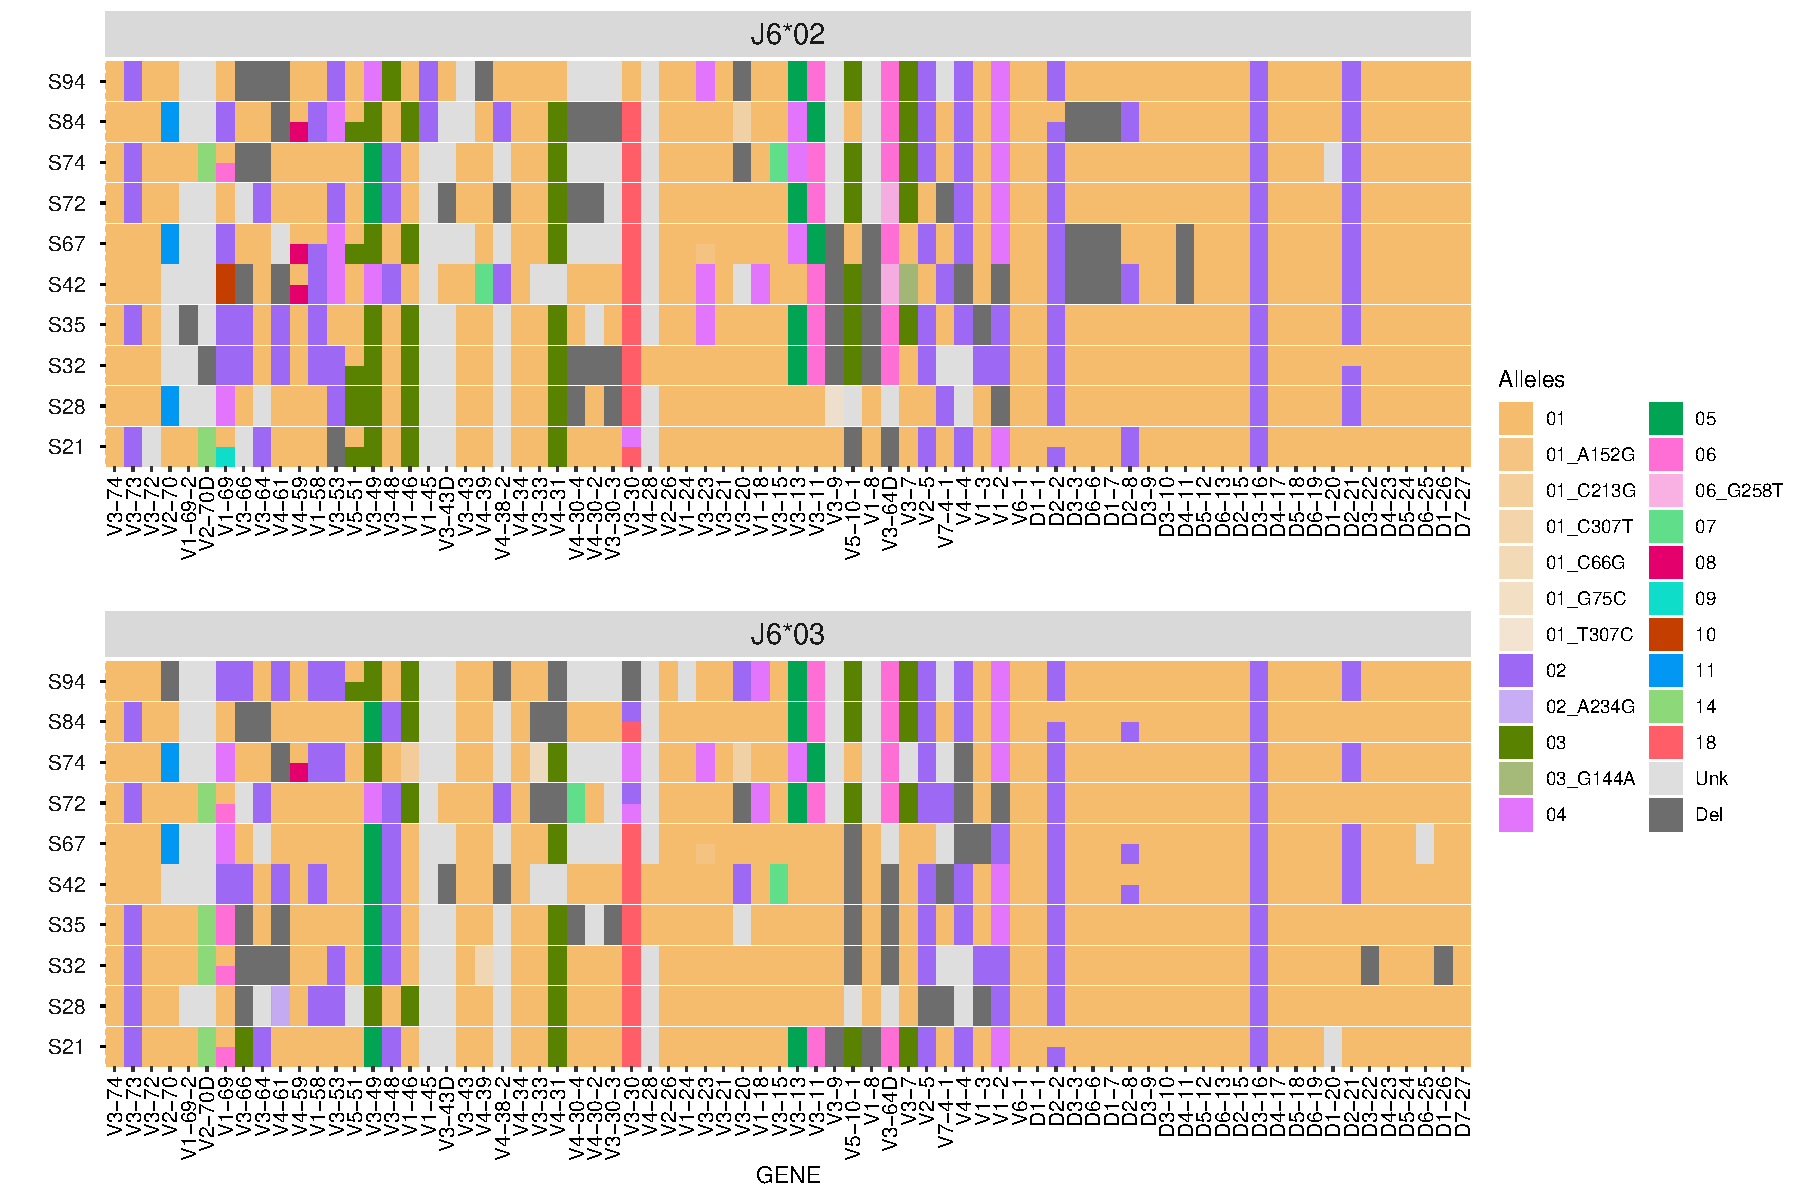
\includegraphics{RAbHIT-vignette_files/figure-latex/unnamed-chunk-6-1.pdf}

The detection of double chromosome deltion from the function can be then
used for the haplotype infernce, this prior knowldege of deletion can
rise the certentiy level of the infrence of the genes where a deletion
where a deletion was detected. The \texttt{createFullHaplotype} recives
a vector of the deleted genes detected. V gene labels marked in red
represent low expressed genes for which deletions are inferred with low
certainty. D gene labels marked in purple represent indistinguishable
genes due to high sequence similarity, therefore alignment call is less
reliable.

\begin{Shaded}
\begin{Highlighting}[]
\CommentTok{# Infered deletion summary table}
\NormalTok{del_binom_db <-}\StringTok{ }\KeywordTok{deletionsByBinom}\NormalTok{(sample_db)}
\NormalTok{haplo_db <-}\StringTok{ }\KeywordTok{createFullHaplotype}\NormalTok{(sample_db,}\DataTypeTok{toHap_col=}\KeywordTok{c}\NormalTok{(}\StringTok{"V_CALL"}\NormalTok{,}\StringTok{"D_CALL"}\NormalTok{),}
\DataTypeTok{hapBy_col=}\StringTok{"J_CALL"}\NormalTok{,}\DataTypeTok{hapBy=}\StringTok{"IGHJ6"}\NormalTok{,}\DataTypeTok{toHap_GERM=}\KeywordTok{c}\NormalTok{(HVGERM,HDGERM),}\DataTypeTok{deleted_genes =}\NormalTok{ del_binom_db,}\DataTypeTok{supress_print =}\NormalTok{ T)}
\KeywordTok{plotHaplotype}\NormalTok{(haplo_db)}
\end{Highlighting}
\end{Shaded}


\includegraphics{RAbHIT-vignette_files/figure-latex/unnamed-chunk-7-1.pdf}

\hypertarget{haplotype-inference-deletion-heatmap}{%
\subsubsection{Haplotype inference deletion
heatmap}\label{haplotype-inference-deletion-heatmap}}

For a group of individuals, the deletions detected by the haplotyping
process can be visualized with \texttt{deletionHeatmap}. The function
create a heatmap of the deletion inferred and colors them by the
certainty level (\(lK\)).

\begin{Shaded}
\begin{Highlighting}[]
\CommentTok{# Load example sequence data}
\KeywordTok{data}\NormalTok{(samples_db)}
\CommentTok{# Infered haplotype summary table for multiple subjects}
\NormalTok{haplo_db <-}\StringTok{ }\KeywordTok{createFullHaplotype}\NormalTok{(samples_db,}\DataTypeTok{toHap_col=}\KeywordTok{c}\NormalTok{(}\StringTok{"V_CALL"}\NormalTok{,}\StringTok{"D_CALL"}\NormalTok{),}
\DataTypeTok{hapBy_col=}\StringTok{"J_CALL"}\NormalTok{,}\DataTypeTok{hapBy=}\StringTok{"IGHJ6"}\NormalTok{,}\DataTypeTok{toHap_GERM=}\KeywordTok{c}\NormalTok{(HVGERM,HDGERM),}\DataTypeTok{supress_print =}\NormalTok{ T)}
\CommentTok{# plot deletion heatmap}
\KeywordTok{deletionHeatmap}\NormalTok{(haplo_db)}
\end{Highlighting}
\end{Shaded}


\includegraphics{RAbHIT-vignette_files/figure-latex/unnamed-chunk-8-1.pdf}

\hypertarget{infering-dj-single-chromosome-deletion-by-v-pooled-approach}{%
\subsubsection{Infering D/J single chromosome deletion by V pooled
approach}\label{infering-dj-single-chromosome-deletion-by-v-pooled-approach}}

Since \emph{V} gene heterozygosity is extremely common, using \emph{V}
genes as anchors for haplotype inference could dramatically increase the
number of people for which \emph{D} haplotype can be inferred. However,
reliable haplotype inference using \emph{V} genes as anchors requires a
much greater sequencing depth than haplotype inference using J6 gene as
an anchor.

The RAbHIT package offeres a solution to overcome the low number of
sequences that connect a given \emph{V-D} allele pair. The package
function applies an aggregation approach, in which information from
several \emph{V} heterozygous genes can be combined to infer \emph{D}
gene deletions.

The \texttt{deletionsByVpooled} function uses the \emph{V} pooled
approach to detect single chromosomal deletion for \emph{D} and
\emph{J}.

\begin{Shaded}
\begin{Highlighting}[]
\CommentTok{# Infered deletion summary table}
\NormalTok{del_db <-}\StringTok{ }\KeywordTok{deletionsByVpooled}\NormalTok{(samples_db)}
\end{Highlighting}
\end{Shaded}

\begin{verbatim}
## [1] "5093 sequnces were removed due to multiple assignments, 37749 sequences left"
## [1] "The following genes used for pooled deletion detection"
##  [1] "IGHV3-23" "IGHV3-15" "IGHV1-18" "IGHV2-5"  "IGHV3-53" "IGHV4-39"
##  [7] "IGHV1-69" "IGHV3-7"  "IGHV3-11" "IGHV3-49"
## [1] "5774 sequnces were removed due to multiple assignments, 29869 sequences left"
## [1] "The following genes used for pooled deletion detection"
## [1] "IGHV3-23" "IGHV3-48" "IGHV5-51" "IGHV1-18" "IGHV3-49" "IGHV1-46"
## [7] "IGHV3-73"
## [1] "5374 sequnces were removed due to multiple assignments, 34009 sequences left"
## [1] "The following genes used for pooled deletion detection"
## [1] "IGHV1-18"  "IGHV1-46"  "IGHV3-64D" "IGHV3-49"  "IGHV2-5"  
## [1] "5884 sequnces were removed due to multiple assignments, 29681 sequences left"
## [1] "The following genes used for pooled deletion detection"
## [1] "IGHV3-30" "IGHV3-48" "IGHV3-7"  "IGHV3-11" "IGHV3-49" "IGHV1-46"
## [1] "3954 sequnces were removed due to multiple assignments, 28840 sequences left"
## [1] "The following genes used for pooled deletion detection"
## [1] "IGHV3-9"  "IGHV1-69" "IGHV3-73"
## [1] "8991 sequnces were removed due to multiple assignments, 44838 sequences left"
## [1] "The following genes used for pooled deletion detection"
##  [1] "IGHV3-30"   "IGHV3-48"   "IGHV3-49"   "IGHV4-59"   "IGHV5-10-1"
##  [6] "IGHV5-51"   "IGHV3-53"   "IGHV3-11"   "IGHV1-69"   "IGHV2-70"  
## [11] "IGHV3-73"   "IGHV1-58"  
## [1] "5736 sequnces were removed due to multiple assignments, 40847 sequences left"
## [1] "The following genes used for pooled deletion detection"
## [1] "IGHV3-11" "IGHV4-39" "IGHV1-46" "IGHV5-51" "IGHV3-48" "IGHV3-13"
## [7] "IGHV3-49" "IGHV3-73"
## [1] "5072 sequnces were removed due to multiple assignments, 33204 sequences left"
## [1] "The following genes used for pooled deletion detection"
## [1] "IGHV3-23" "IGHV3-48" "IGHV1-46" "IGHV3-49" "IGHV3-7"  "IGHV3-11"
## [7] "IGHV1-58" "IGHV3-13"
## [1] "1212 sequnces were removed due to multiple assignments, 8737 sequences left"
## [1] "The following genes used for pooled deletion detection"
## [1] "IGHV3-53" "IGHV3-48" "IGHV3-11" "IGHV1-46" "IGHV1-69" "IGHV2-5" 
## [7] "IGHV3-49"
## [1] "3624 sequnces were removed due to multiple assignments, 22412 sequences left"
## [1] "The following genes used for pooled deletion detection"
## [1] "IGHV3-33"   "IGHV3-30"   "IGHV3-15"   "IGHV1-46"   "IGHV3-48"  
## [6] "IGHV3-73"   "IGHV3-49"   "IGHV2-70"   "IGHV5-10-1"
\end{verbatim}

\begin{Shaded}
\begin{Highlighting}[]
\KeywordTok{head}\NormalTok{(del_db)}
\end{Highlighting}
\end{Shaded}

\begin{verbatim}
##       GENE DELETION   K1_NEW COUNTS1_NEW    V_GENE     K1 SUBJECT
## 1  IGHD1-1        0 19.08503       15,22 V(pooled)  19.09     S42
## 2 IGHD1-20        0 12.03093       10,17 V(pooled)  12.03     S42
## 3 IGHD1-26        0 39.61305     330,564 V(pooled)  39.61     S42
## 4  IGHD1-7        1  8.22609        7,68 V(pooled)   8.23     S42
## 5 IGHD2-15        0 198.5908     170,309 V(pooled) 198.59     S42
## 6  IGHD2-2        0 279.3872     234,405 V(pooled) 279.39     S42
\end{verbatim}

For visualzing the deletion detected by \texttt{deletionsByVpooled}, the
\texttt{plotDeletionsByVpooled} can be used. However, it is recomended
to use this function for multiple individuals.

\begin{Shaded}
\begin{Highlighting}[]
\CommentTok{# Plot the deletion heatmap}
\KeywordTok{plotDeletionsByVpooled}\NormalTok{(del_db)}
\end{Highlighting}
\end{Shaded}


\includegraphics{RAbHIT-vignette_files/figure-latex/unnamed-chunk-10-1.pdf}

\hypertarget{references}{%
\subsection{References}\label{references}}

\begin{enumerate}
\def\labelenumi{\arabic{enumi}.}
\tightlist
\item
  \href{https://doi.org/10.1101/314476}{Gidoni \emph{et al.} (2018)}.
\item
  \href{https://doi.org/10.1101/405704}{Gadala-Maria and Gidoni \emph{et
  al.} (2018)}
\item
  \href{http://www.ncbi.nlm.nih.gov/pubmed/20147303}{Munshaw and Kepler
  (2010)}
\item
  \href{http://www.ncbi.nlm.nih.gov/pubmed/12477501}{Lefranc \emph{et
  al.} (2003)}
\item
  \href{http://doi.org/10.1093/bioinformatics/btv359}{Gupta \emph{et
  al.} (2015)}
\end{enumerate}


\end{document}
